\documentclass[12pt]{article}
\setlength{\parindent}{0in}
\setlength{\parskip}{\baselineskip}

\usepackage[top=0.75in, bottom=0.75in, left=1in, right=1in]{geometry}

\usepackage{amsmath,amsfonts,amssymb,graphicx, hyperref, float, multirow}

\begin{document}

IBEHS 4A03 \hfill Assignment \#4\\
Baoze Lin, Hady Ibrahim

\hrulefill

% Custom numbering for subparts (e.g., 2.1, 2.2)
\renewcommand{\theenumii}{\arabic{enumi}.\arabic{enumii}}

\begin{enumerate}
  \item Question 1
    \begin{enumerate}
    
      % Answer to 1.1
      \item 
      The Routh array was constructed by first rewriting the characteristic equation of the closed-loop system using the substitution $T_I = \frac{1}{\tau_I}$ to simplify the algebra. The goal was to determine the range of $K_C$ and $\tau_I$ values that lead to a stable system based on Routh-Hurwitz criteria.
  
      \begin{figure}[H]
        \centering
        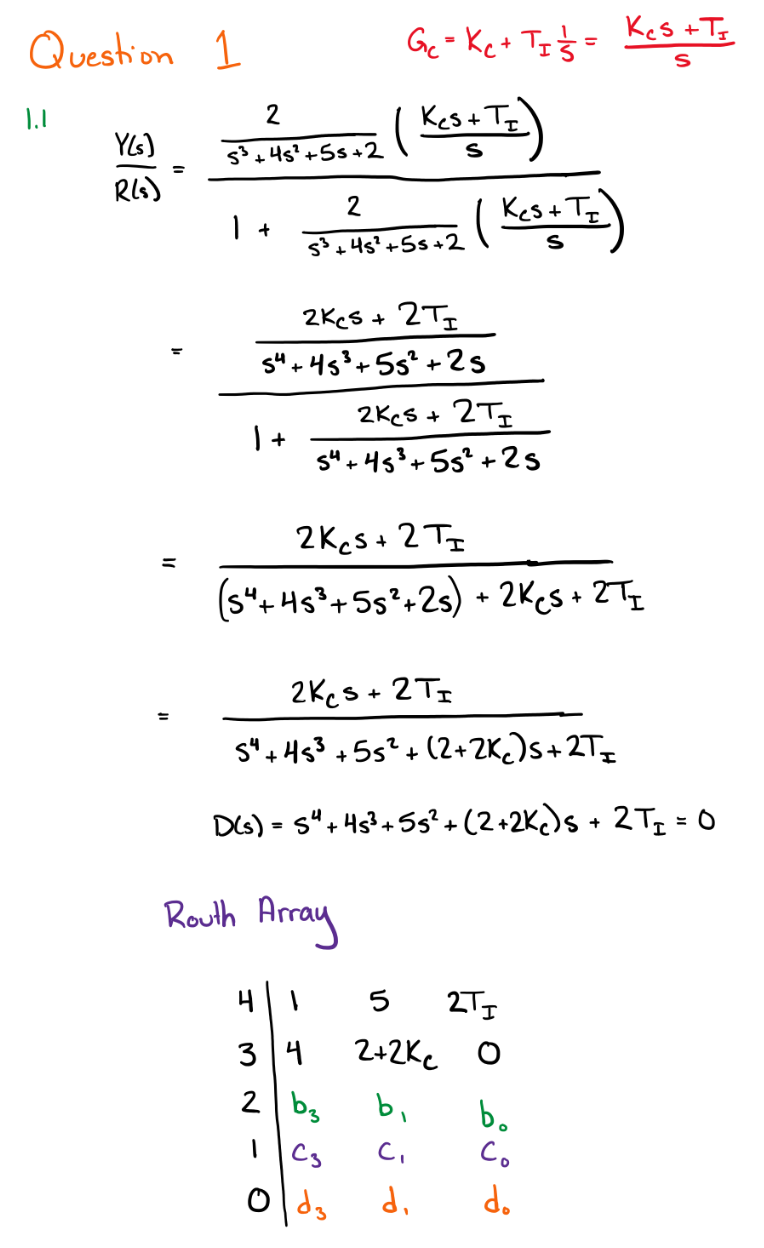
\includegraphics[width=0.6\textwidth]{Figures/figure1-1a.png}
        \caption{Step 1 of Routh Array derivation.}
      \end{figure}
  
      \begin{figure}[H]
        \centering
        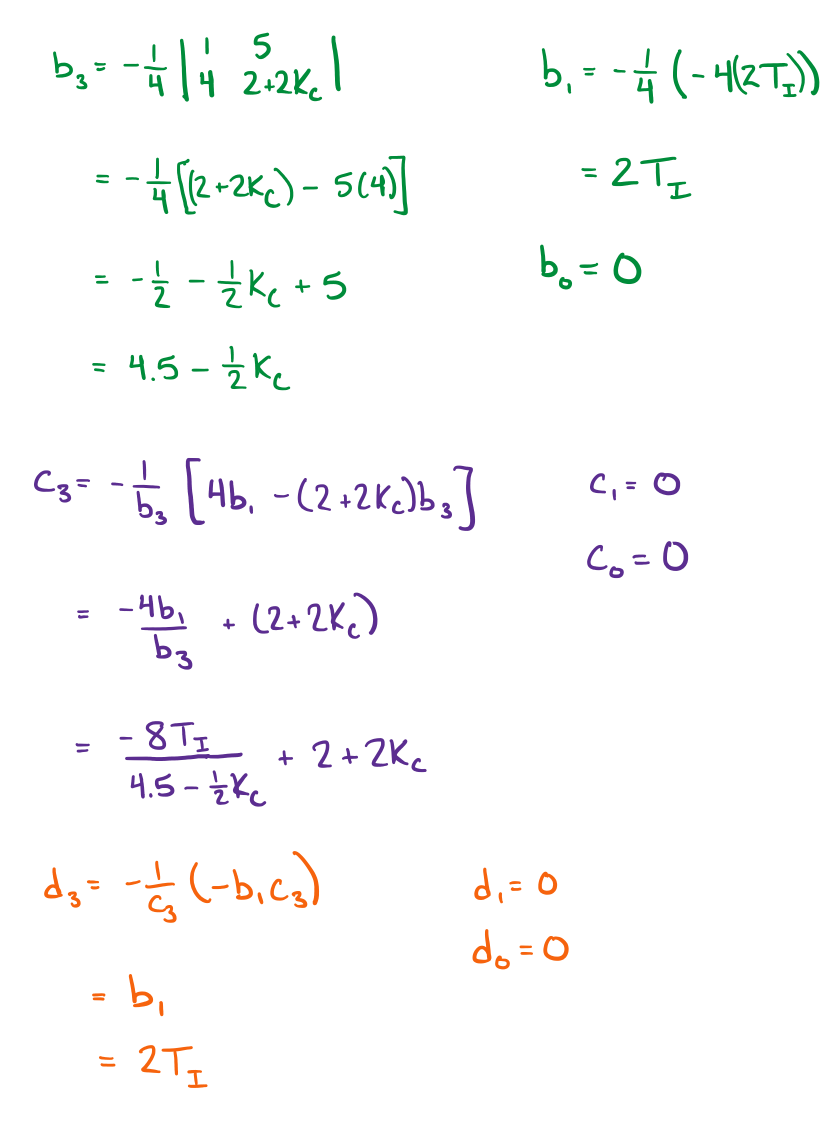
\includegraphics[width=0.7\textwidth]{Figures/figure1-1b.png}
        \caption{Step 2 of Routh Array derivation.}
      \end{figure}
  
      \begin{figure}[H]
        \centering
        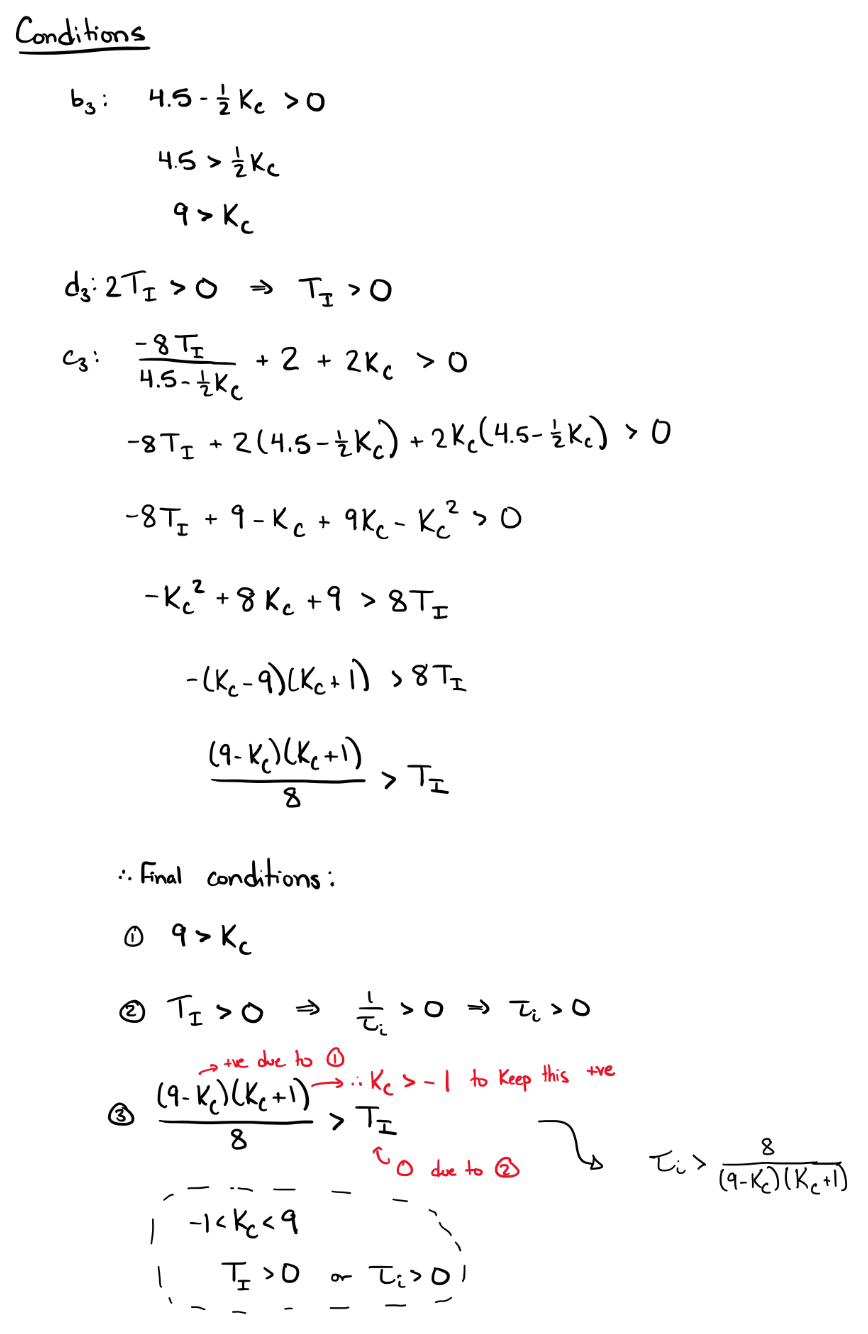
\includegraphics[width=0.7\textwidth]{Figures/figure1-1c.png}
        \caption{Final Routh Array with derived inequalities for stability.}
      \end{figure}
  
      \clearpage
      % Answer to 1.2
      \item 
      Using the inequalities derived in 1.1, the feasible set was plotted to visualize combinations of $K_C$ and $\tau_I$ that result in closed-loop stability. The red shaded region indicates infeasible (unstable) parameter combinations.
  
      \begin{figure}[H]
        \centering
        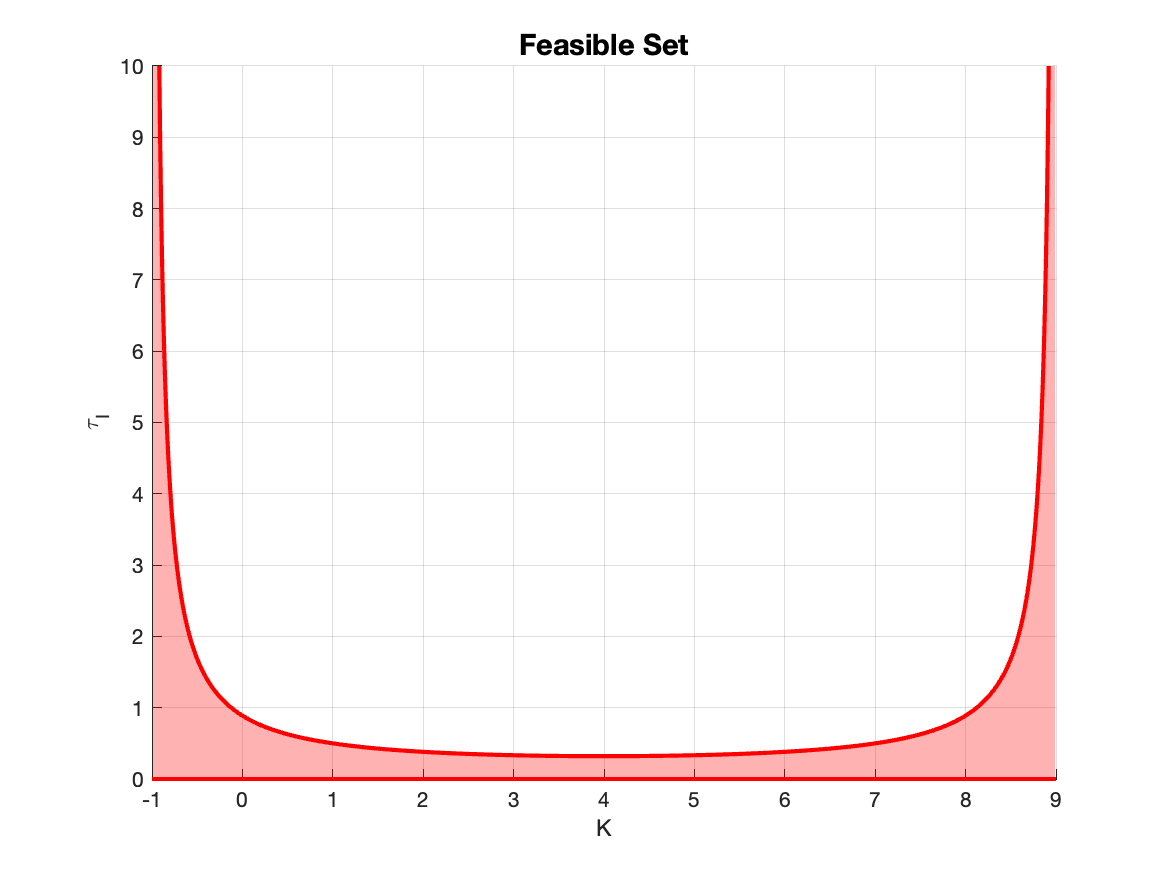
\includegraphics[width=0.8\textwidth]{Figures/figure1-2a.png}
        \caption{Feasible set for $K_C$ and $\tau_I$ from Routh-Hurwitz conditions.}
      \end{figure}
  
      % Answer to 1.3
      \item 
      A Simulink model was developed to simulate the closed-loop response of the system. Three scenarios were tested: one inside the feasible region, one outside, and one on the edge.
  
      \begin{figure}[H]
        \centering
        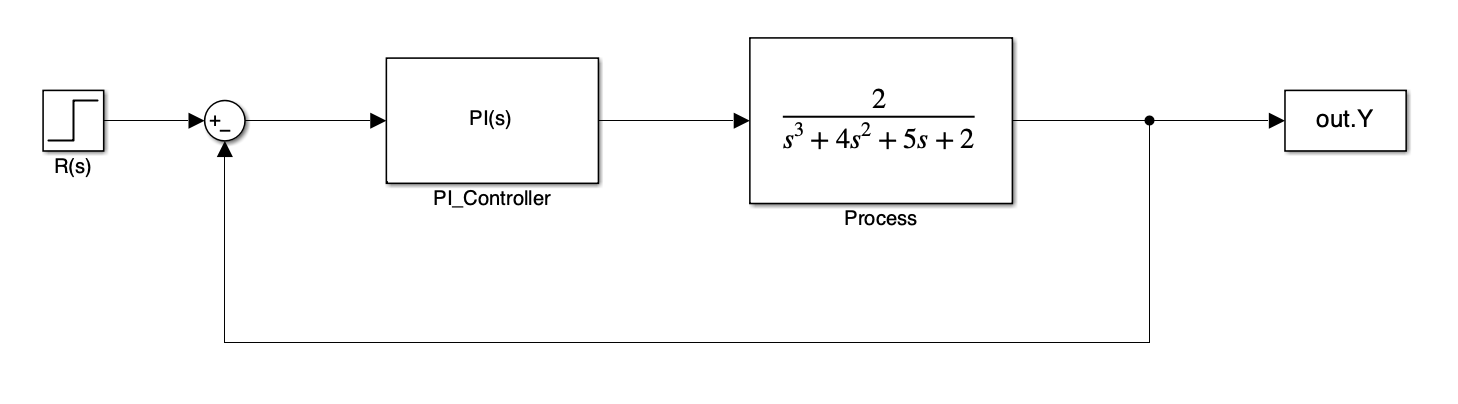
\includegraphics[width=1\textwidth]{Figures/figure1-3a.png}
        \caption{Simulink model of the PI-controlled system.}
      \end{figure}

      \begin{figure}[H]
        \centering
        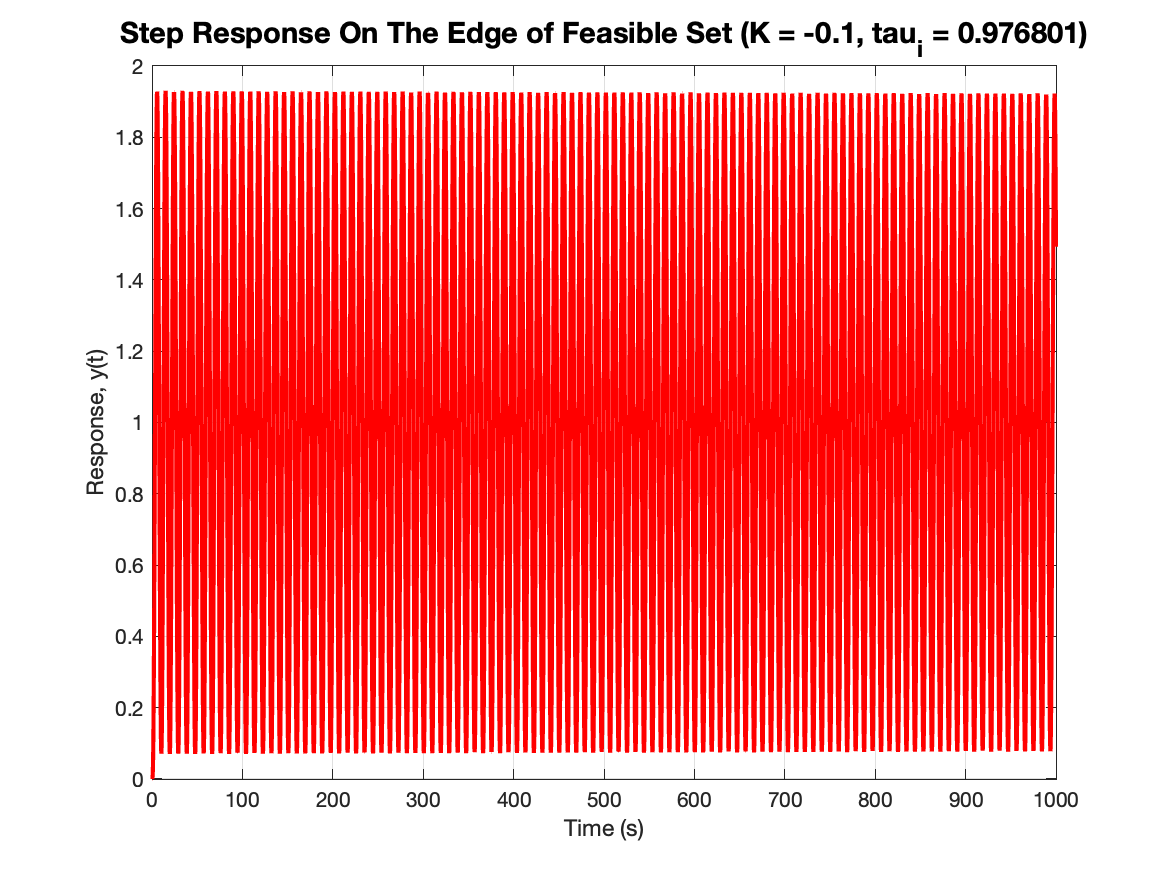
\includegraphics[width=0.7\textwidth]{Figures/figure1-3b.png}
        \caption{Step response on the boundary of the feasible set. The system oscillates and the amplitude grows very slowly, indicating marginal instability.}
      \end{figure}
      
      \begin{figure}[H]
        \centering
        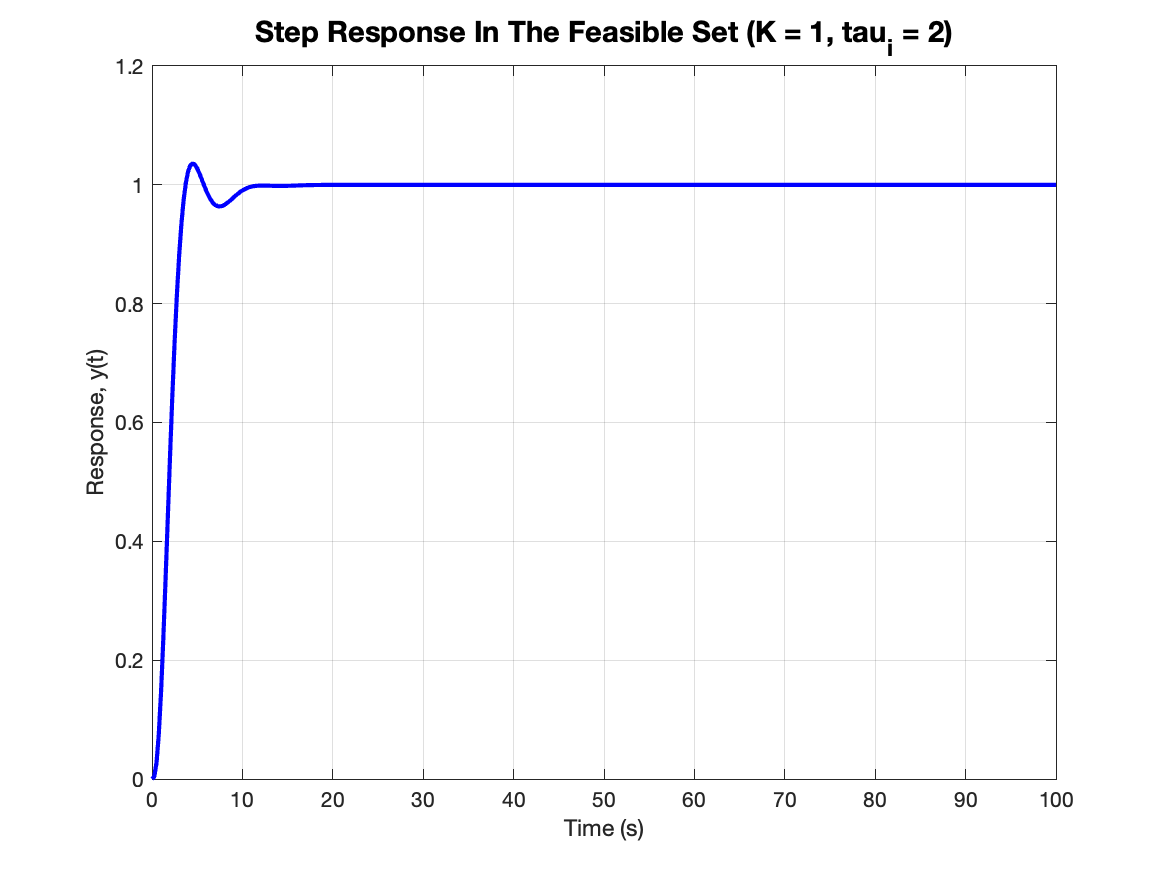
\includegraphics[width=0.7\textwidth]{Figures/figure1-3c.png}
        \caption{Step response for parameters inside the feasible set. The system is stable and relatively well damped, approaching steady state smoothly.}
      \end{figure}
      
      \begin{figure}[H]
        \centering
        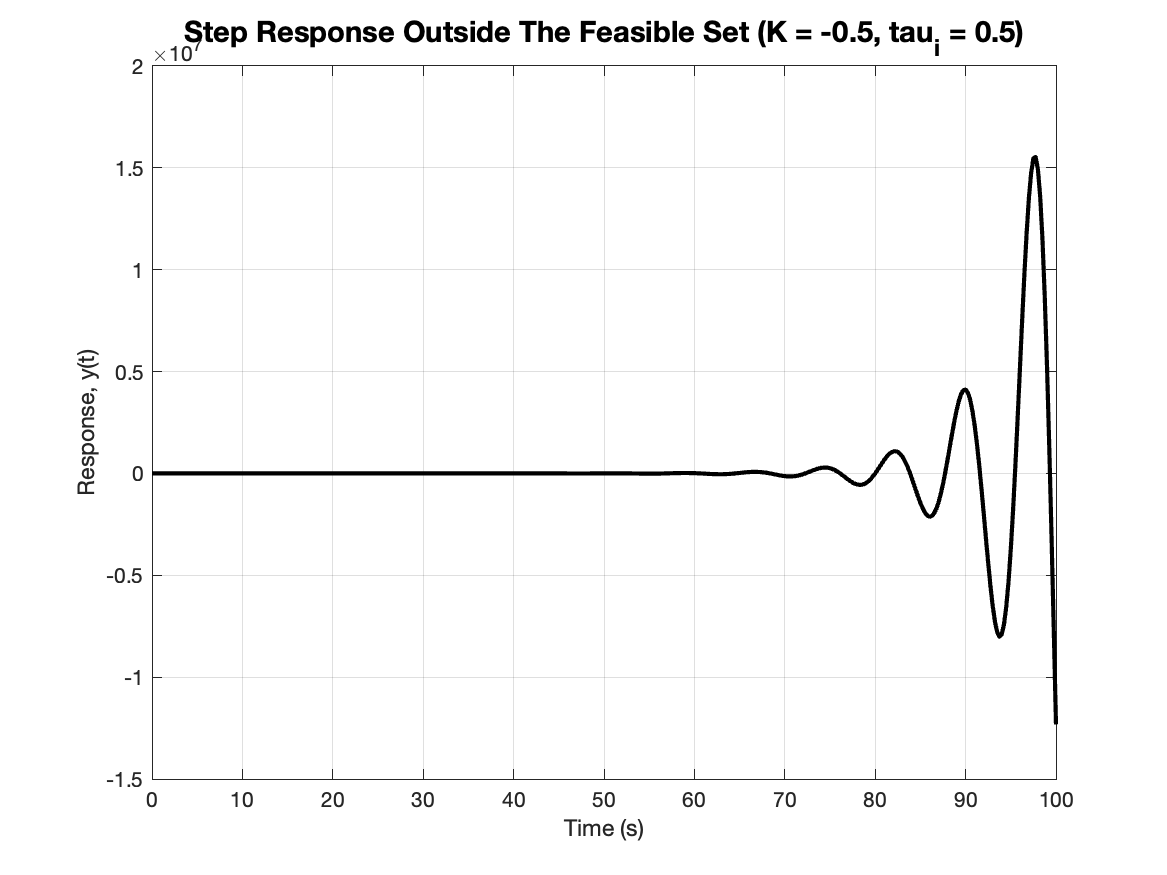
\includegraphics[width=0.7\textwidth]{Figures/figure1-3d.png}
        \caption{Step response for parameters outside the feasible set. The system exhibits fast-growing oscillations, clearly demonstrating instability.}
      \end{figure}
      
      The edge case exhibits slow-growing oscillations, which indicates marginal instability. Although the system initially appears to behave stably, the oscillations increase in amplitude over time. This is consistent with the fact that the chosen parameters lie directly on the boundary of the feasible set, where the Routh-Hurwitz conditions require strict inequalities ($>$) rather than allowing equality. The second case, which is well within the feasible region, produces a stable and mostly well-damped response. The final case, with parameters outside the feasible set, immediately shows rapidly growing oscillations, confirming instability.

      \clearpage
      % Answer to 1.4
      \item 
      The Routh-Hurwitz array was recomputed with the new transport delay (using first-order Padé approximation) to determine how the delay affects system stability.
  
      \begin{figure}[H]
        \centering
        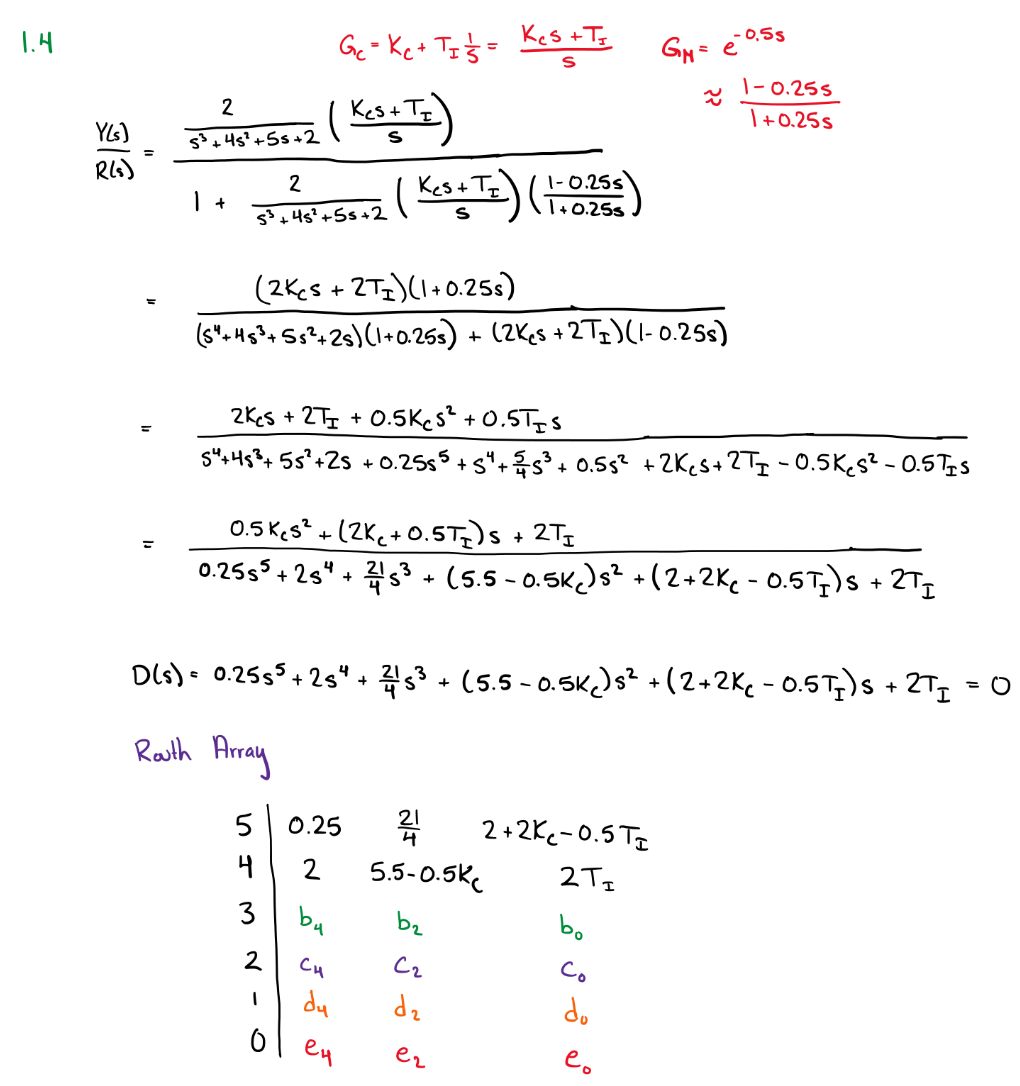
\includegraphics[width=0.9\textwidth]{Figures/figure1-4a.png}
        \caption{Step 1 of Routh Array with transport delay.}
      \end{figure}
  
      \begin{figure}[H]
        \centering
        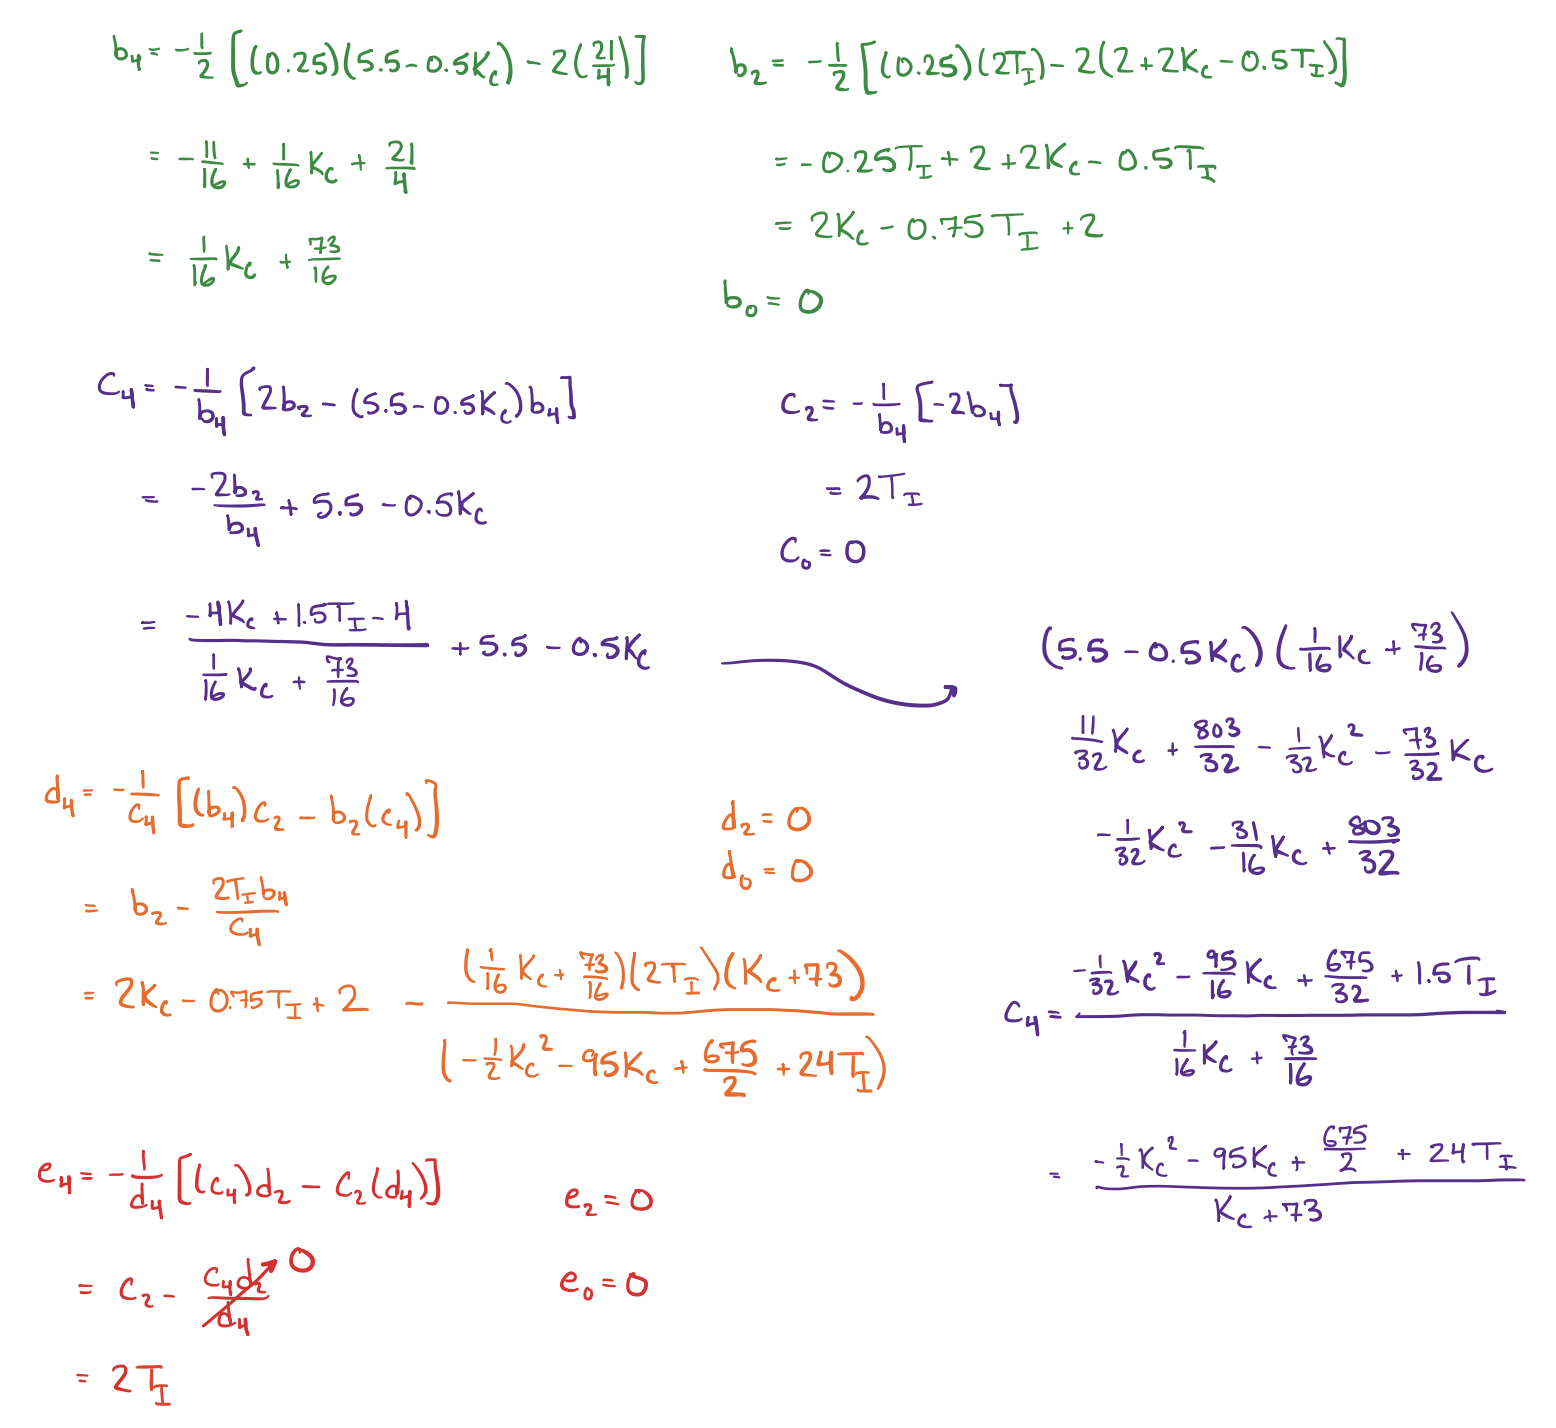
\includegraphics[width=0.9\textwidth]{Figures/figure1-4b.png}
        \caption{Step 2 of Routh Array with transport delay.}
      \end{figure}
  
      \begin{figure}[H]
        \centering
        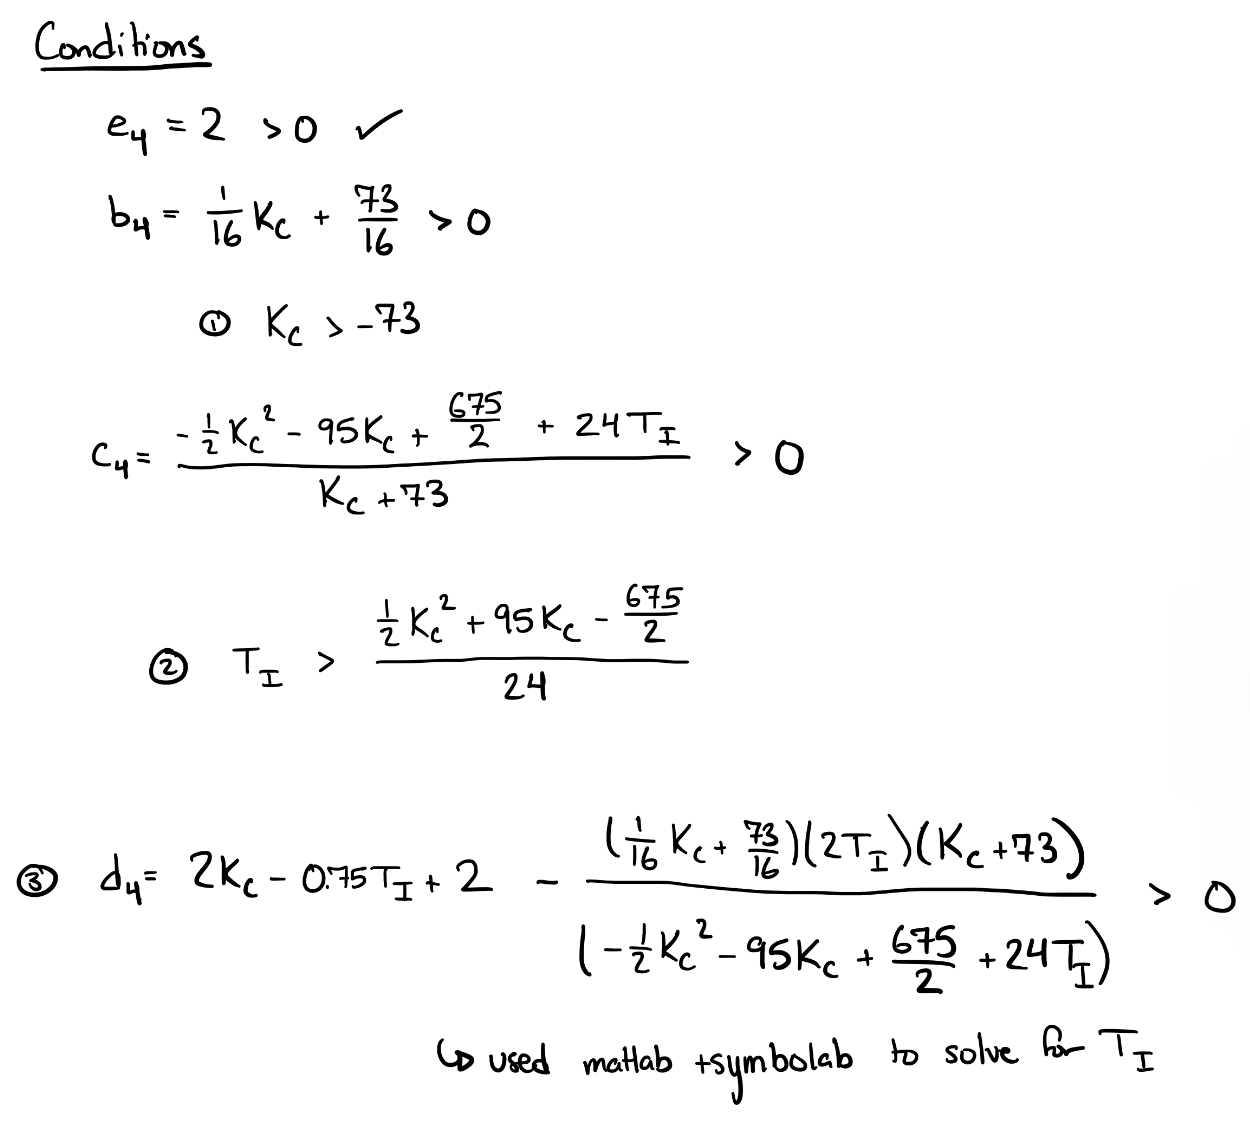
\includegraphics[width=0.8\textwidth]{Figures/figure1-4c.png}
        \caption{Final Routh Array with delay-based conditions.}
      \end{figure}
  
      \begin{figure}[H]
        \centering
        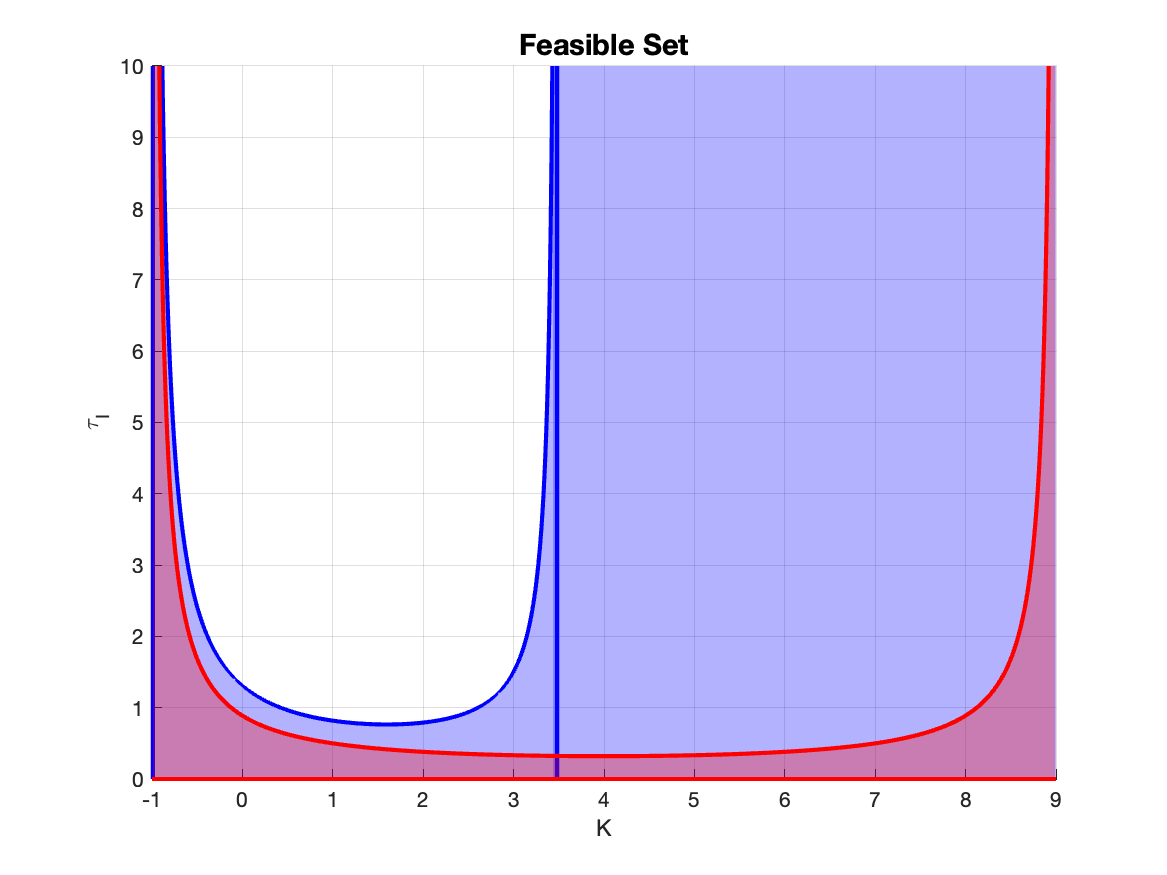
\includegraphics[width=0.8\textwidth]{Figures/figure1-4d.png}
        \caption{Feasible sets with and without delay. Blue indicates infeasible region of the new delayed system. Red is the same infeasible region from earlier.}
      \end{figure}
  
      As seen in the figure, the introduction of transport delay reduces the size of the feasible region, particularly in areas with small integral time $\tau_I$ or large controller gain $K_C$. This is because transport delay introduces additional phase lag into the system, which decreases the phase margin and brings the system closer to instability. From the perspective of the Bode plot, delay shifts the phase curve to the left, meaning that the phase crosses $-180^\circ$ at a lower frequency. This corresponds to a higher critical gain $A_c$, which implies a lower allowable $K_C$ for stability. In practical terms, this means that the system must be detuned ($K_C$ must be reduced) when delay is present. If the gain is not reduced accordingly, the aggressive controller action causes excessive oscillations, and the system approaches instability. This explains why many of the previously stable combinations of $K_C$ and $\tau_I$ now fall outside the feasible set when delay is introduced.

      \clearpage
      % Answer to 1.5
      \item 
      The system was simulated again using the same controller parameters ($K_C=2$, $\tau_I=1$) for both the delay and non-delay versions. These values were chosen by looking at the feasible sets and picking values that lay in both the time delay and non-time delayed feasible sets. The updated Simulink model includes the transport delay block.
  
      \begin{figure}[H]
        \centering
        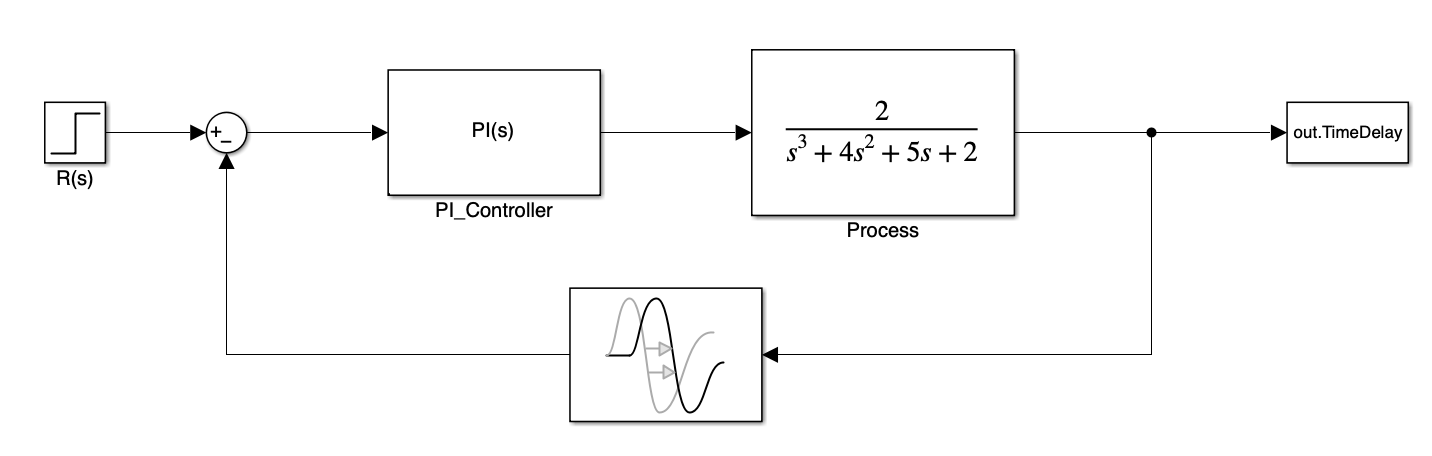
\includegraphics[width=0.9\textwidth]{Figures/figure1-5a.png}
        \caption{Simulink model with transport delay included.}
      \end{figure}
  
      \begin{figure}[H]
        \centering
        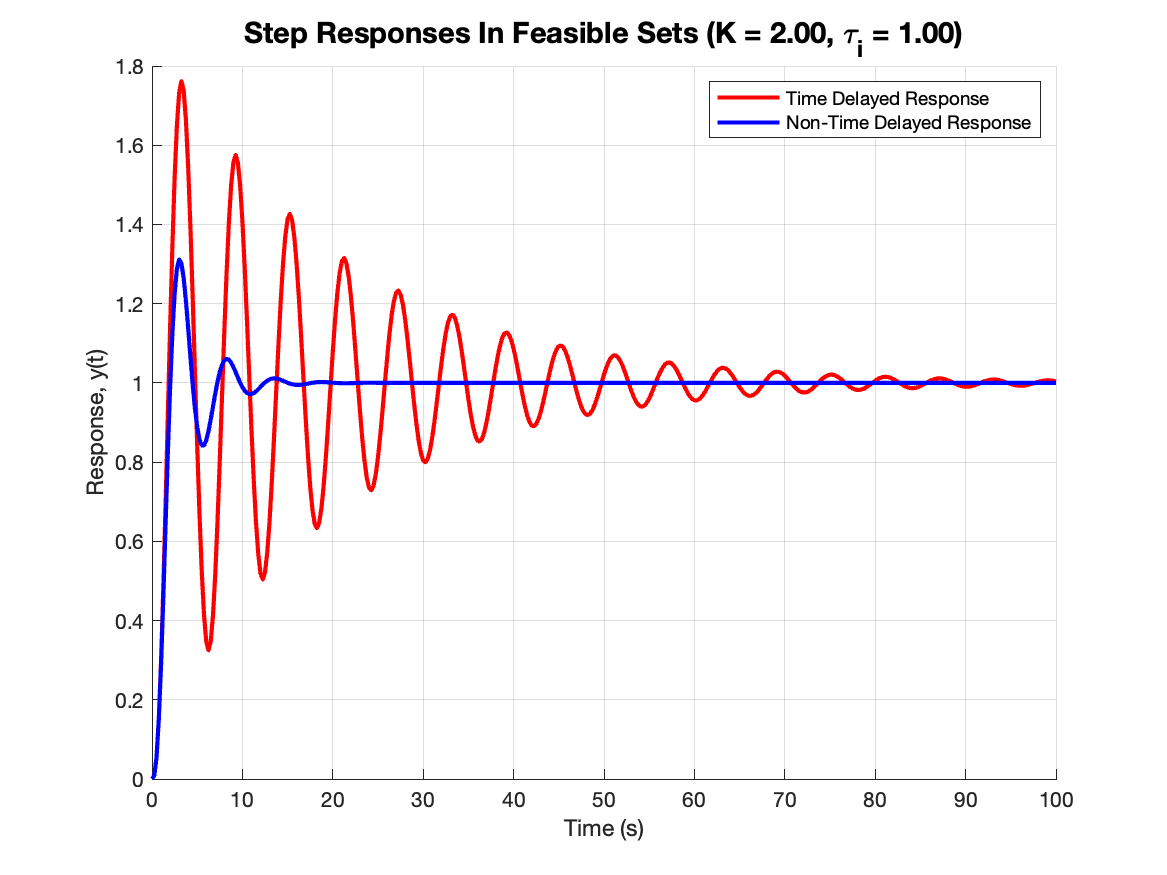
\includegraphics[width=0.8\textwidth]{Figures/figure1-5b.png}
        \caption{Comparison of system response with and without transport delay.}
      \end{figure}
  
      The system with transport delay exhibits more oscillatory behavior and takes longer to settle compared to the delay-free case, despite using identical PI tuning parameters. This aligns with the analysis in 1.4, where the added phase lag from delay was shown to reduce stability margins and narrow the feasible set. The delay effectively pushes the system closer to instability, and without detuning $K_C$, even stable configurations become more oscillatory and sluggish in response.  
    \end{enumerate}
    

\clearpage
\item Question 2
  \begin{enumerate}
    % 2.1
    \item 
    The approximated first-order system equation for the closed-loop system is given by:
    
    \begin{equation}
      \frac{Y(s)}{U(s)} = \frac{-1.2e^{-5s}}{6s + 1} = \frac{Ke^{-\theta s}}{\tau s + 1}
    \end{equation}

    We first start with the \textbf{Cohen-Coon} heuristic. From class, we are given the following equations:

    $$
      K_C = \frac{1}{K} \cdot \frac{\tau}{\theta} \left( \frac{4}{3} + \frac{\theta}{4\tau} \right) \quad \quad \quad \quad \quad
      \tau_I = \theta \cdot \frac{32 + \frac{6\theta}{\tau}}{13 + \frac{8\theta}{\tau}} \quad \quad \quad \quad \quad
      K_D = \theta \cdot \frac{4}{11 + \frac{2\theta}{\tau}} \\
    $$

    We thus get the answers below:

    \[
    K_c = \frac{1}{\left(-1.2\right)} \left( \frac{6}{5} \right) \left( \frac{4}{3} + {\frac{5}{4 \cdot 6}} \right) = -1.54166
    \]

    \[
      \tau_I = \left(5\right) \cdot \frac{32 + \frac{6\left(5\right)}{\left(6\right)}}{13 + \frac{8\left(5\right)}{\left(6\right)}} = 9.40677
    \]

    \[
      K_D = \left(5\right) \cdot \frac{4}{11 + \frac{2\left(5\right)}{\left(6\right)}} = 1.5789
    \]

    We then move onto the \textbf{Ciancone} heuristic. Since this system is for setpoint tracking, we use the correlation graphs as shown in class. To avoid wasting digital ink, the graphs were not attached.

    For all graphs, we need to derive the fraction dead time first:

    \[
      \frac{\theta}{\theta + \tau} = \frac{5}{5 + 6} = 0.454545
    \]

    For the graphs \( K_c K_p \), \( \frac{\tau_I}{\theta + \tau} \), and \( \frac{K_D}{\theta + \tau} \), we get the values 0.73, 0.73, and 0.08 respectively. Solving for \( K_c \), \( \tau_I \), and \( K_D \) gives us:

    $$
      K_C = \frac{0.73}{-1.2} = -0.683 \quad \quad \quad \quad \quad
      \tau_I = \left(5 + 6\right) \cdot 0.73 = 8.03 \quad \quad \quad \quad \quad
      K_D = \left(5 + 6\right) \cdot 0.08 = 0.88 \\
    $$

    \pagebreak

    Lastly, we calculate the \textbf{ITAE} heuristic. We start with the equation:

    \[
      Y = A\left(\frac{\theta}{\tau}\right)^B
    \]

    The values of \( A \) and \( B \) are given in the table below:

    \begin{table}[H]
      \centering
      \begin{tabular}{|c|c|c|c|}
      \hline
      \textbf{Controller} & \textbf{Mode} & \textbf{A} & \textbf{B} \\
      \hline
      \multirow{3}{*}{PID} & P & 0.965 & -0.85 \\
                           & I & 0.796 & -0.1465 \\
                           & D & 0.308 &  0.929 \\
      \hline
      \end{tabular}
      \caption{Controller Parameters A and B for PID Mode}
    \end{table}

    We also note the following equations to calculate the parameters in set-point tracking:

    \[
    Y_P = KK_C \quad \quad \quad \quad \quad
    Y_I = \frac{\tau}{\tau_I} = A + B \left( \frac{\theta}{\tau} \right) \quad \quad \quad \quad \quad
    Y_D = \frac{K_D}{\tau}
    \]

    We do some mathematics:

    $$
      Y_P = \left(0.965\right)\left(\frac{\theta}{\tau}\right)^{-0.85} = 1.12675 \quad \quad \quad 
      K_C = \frac{1.12675}{-1.2} = -0.938958
    $$

    $$
      Y_I = \left(0.796\right) + \left(-0.1465\right) \cdot \left(\frac{\theta}{\tau}\right) = 0.67391 \quad \quad \quad 
      \tau_I = \frac{6}{0.67391} = 8.895
    $$
    $$
      Y_D = \left(0.308\right)\left(\frac{\theta}{\tau}\right)^{0.929} = 0.26001 \quad \quad \quad 
      K_D = 0.26001 \cdot 6 = 1.56006
    $$

    % 2.2
    \item
    The Bode plot is shown below in Figure \ref{fig:figure2_2}.

    \begin{figure}[H]
      \centering
      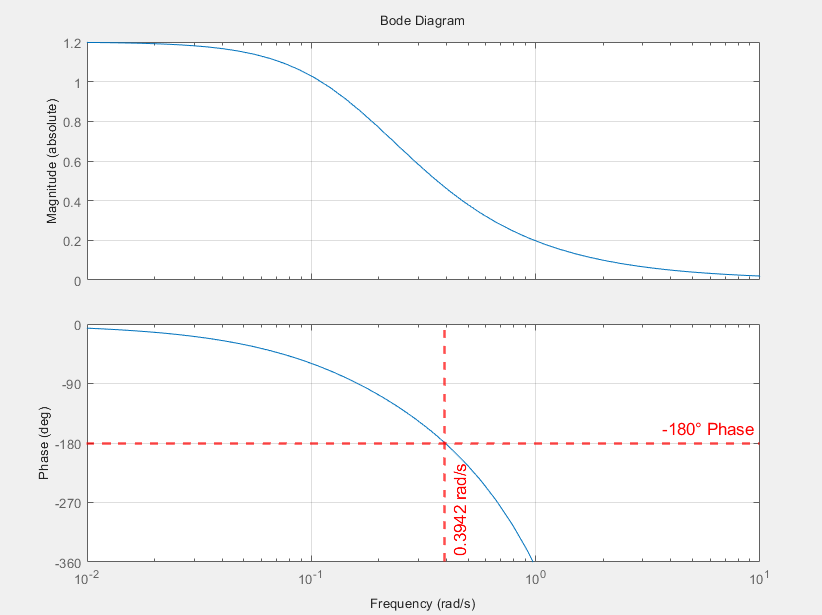
\includegraphics[width=\textwidth]{Figures/figure2-2.png}
      \caption{Bode plot of the closed-loop system with transport delay.}
      \label{fig:figure2_2}
    \end{figure}

    From the Bode plot and the associated Matlab code, we derive the Critical Frequency and the amplitude at said frequency as 0.3942 rad/s and 0.4673. With these numbers, we calculate the ultimate gain and the ultimate period.

    \[
    K_u = \frac{1}{\text{Critical Amplitude}} = \frac{1}{0.3942} \approx 2.537
    \]

    \[
    T_u = \frac{2\pi}{\omega_c} = \frac{2\pi}{0.4673} \approx 13.445
    \]

    We then calculate the PID parameters $K_c$, $\tau_I$ and $K_D$ using the Ziegler-Nichols tuning rules.

    \[
    K_c = \frac{-K_u}{1.7} = \frac{-2.537}{1.7}\approx -1.492
    \]

    \[
    \tau_I = \frac{T_u}{2} = \frac{13.445}{2} \approx 6.7225
    \]

    \[
    K_D = \frac{T_u}{8} = \frac{13.445}{8} \approx 1.6806
    \]

    % 2.3
    \item
    Looking at the Figure \ref{fig:figure2_3a} and Figure \ref{fig:figure2_3e}, the Cohen-Coon controller exhibits a more aggressive and sharp transition. Its initial decrease is steeper and reaches a larger negative value compared to the other controllers. This behavior is likely due to the high values of $K_p$ and $K_d$ within the controller. Additionally, the Cohen-Coon controller takes the longest time to converge, requiring close to 70 hours to stabilize.

    In contrast, the Ciancone controller Figure \ref{fig:figure2_3b} produces an output that resembles an overdamped response. While it is slower to converge compared to the ITAE and Ziegler-Nichols controllers, it is still faster than the Cohen-Coon controller, stabilizing in approximately 40 hours.

    The ITAE controller (Figure \ref{fig:figure2_3c}) stands out for its faster convergence and smaller overshoot compared to the other designs. Its response is smooth and stable, making it an efficient choice. 
    
    The Ziegler-Nichols controller (Figure \ref{fig:figure2_3d})follows a similar shape to the ITAE controller but exhibits a greater overshoot and more pronounced oscillations.

    Based on the analysis of all the graphs, the ITAE controller demonstrates the best overall performance among the four designs, offering a balance of speed, stability, and minimal overshoot.

    \begin{figure}[H]
      \centering
      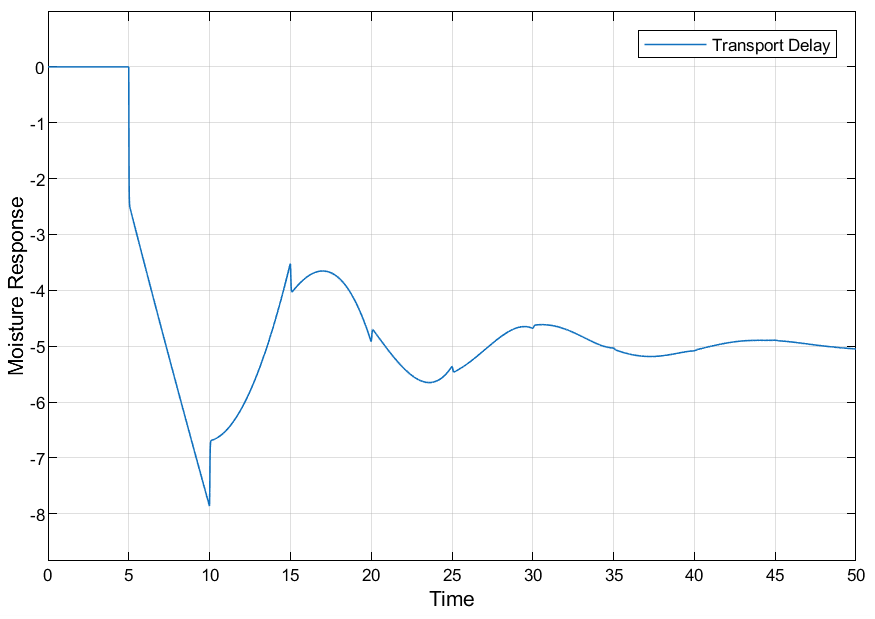
\includegraphics[width=0.7\textwidth]{Figures/figure2-3a.png}
      \caption{Step Response with Cohen-Coon Tuning}
      \label{fig:figure2_3a}
    \end{figure}

    \begin{figure}[H]
      \centering
      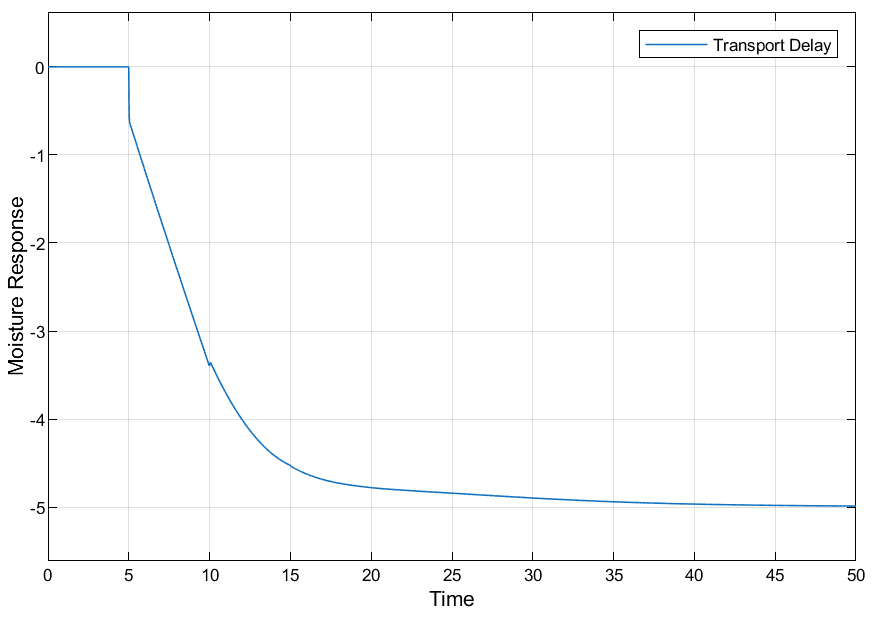
\includegraphics[width=0.7\textwidth]{Figures/figure2-3b.png}
      \caption{Step Response with Ciancone Tuning}
      \label{fig:figure2_3b}
    \end{figure}

    \begin{figure}[H]
      \centering
      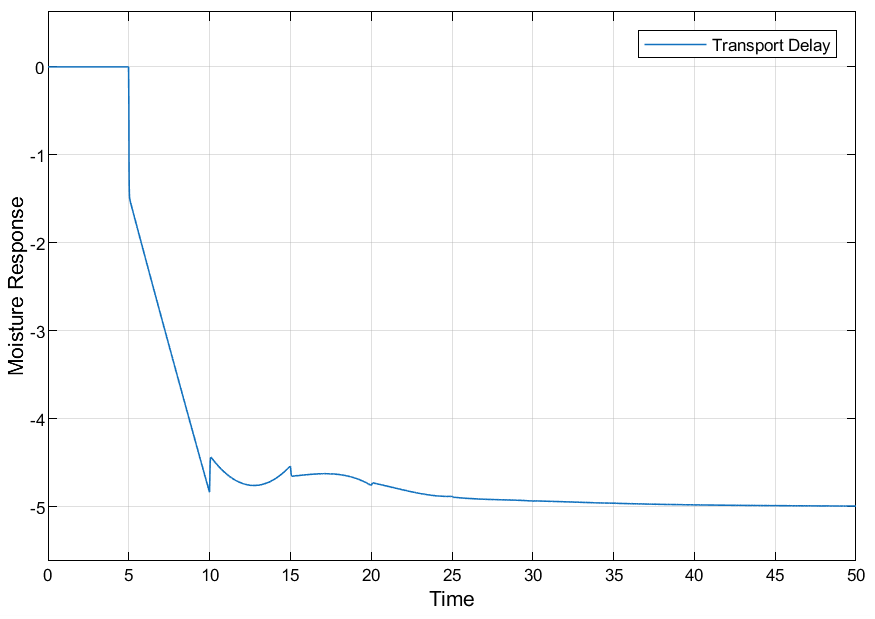
\includegraphics[width=0.7\textwidth]{Figures/figure2-3c.png}
      \caption{Step Response with ITAE Tuning}
      \label{fig:figure2_3c}
    \end{figure}

    \begin{figure}[H]
      \centering
      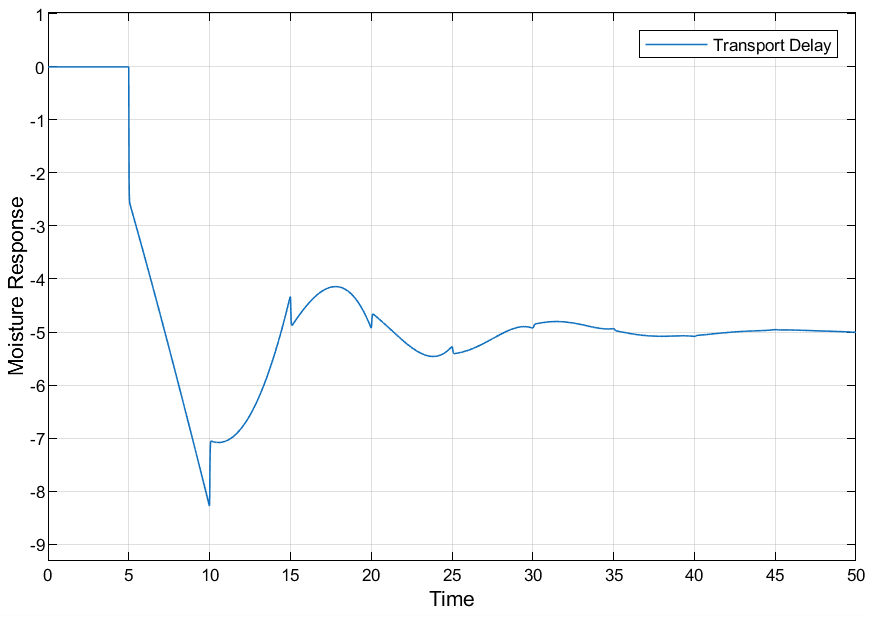
\includegraphics[width=0.7\textwidth]{Figures/figure2-3d.png}
      \caption{Step Response with Ziegler-Nichols Tuning}
      \label{fig:figure2_3d}
    \end{figure}

    \begin{figure}[H]
      \centering
      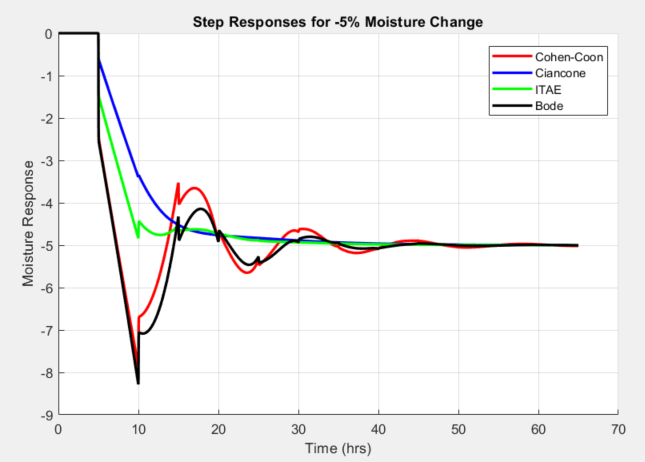
\includegraphics[width=0.7\textwidth]{Figures/figure2-3e.png}
      \caption{Comparison of Step Response with All Tuning}
      \label{fig:figure2_3e}
    \end{figure}

    % 2.4
    \item
    The Integral Squared Error (ISE) is a quantitative metric used to evaluate the performance of a control system. It is defined as:
    \[
    \text{ISE} = \int_0^\infty e^2(t) \, dt
    \]
    where \( e(t) \) is the error signal, calculated as the difference between the desired input and the system output. The ISE penalizes large errors more heavily due to the squared term, making it useful for minimizing overshoot and oscillations in the system response.

    The Integral of Time-weighted Absolute Error (ITAE) is another performance metric, defined as:
    \[
    \text{ITAE} = \int_0^\infty t |e(t)| \, dt
    \]
    Unlike ISE, ITAE penalizes errors that persist over time, encouraging faster convergence and smoother responses. ITAE is particularly useful for optimizing controllers in systems where stability and rapid settling are critical.

    To optimize the PID controller parameters, the derivative gain (\( K_d \)) was fixed at the ITAE value of \( K_d = 1.56006 \), while the proportional gain (\( K_c \)) and integral time (\( \tau_I \)) were varied. The system was simulated for a step change of \(-5\%\) moisture, and the Integral Squared Error (ISE) was calculated for each combination of \( K_c \) and \( \tau_I \).

    Figure \ref{fig:figure2_4a} shows the contour plot of ISE values versus \( K_c \) and \( \tau_I \). The plot reveals a clear region of optimal performance, where the ISE is minimized. The optimal parameters were identified as:
    \[
    K_c = -1.2, \quad \tau_I = 7.5
    \]
    These values correspond to the lowest ISE, indicating the best controller performance in terms of minimizing overshoot, oscillations, and settling time.

    \begin{figure}[H]
      \centering
      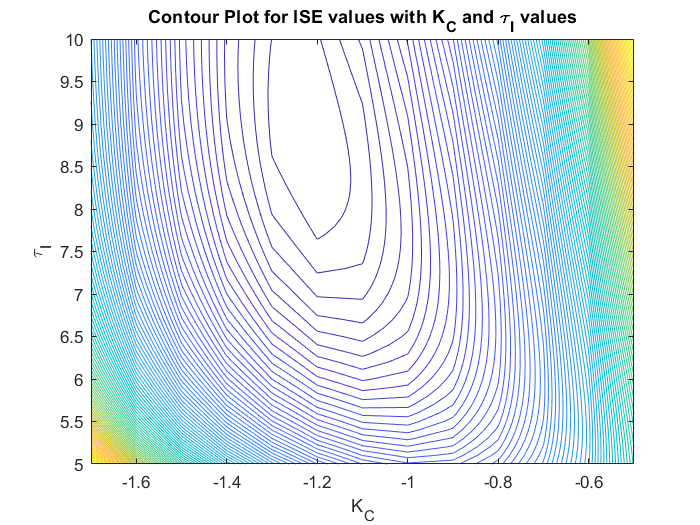
\includegraphics[width=0.7\textwidth]{Figures/figure2-4a.png}
      \caption{Contour Plot of ISE Values for Range of \( K_c \) and \( \tau_I \)}
      \label{fig:figure2_4a}
    \end{figure}

    The system was simulated with the optimal controller and compared to other designs, including Cohen-Coon, Ciancone, ITAE, and Bode controllers. Figure \ref{fig:figure2_4b} shows the step responses for all controllers.

    \begin{figure}[H]
      \centering
      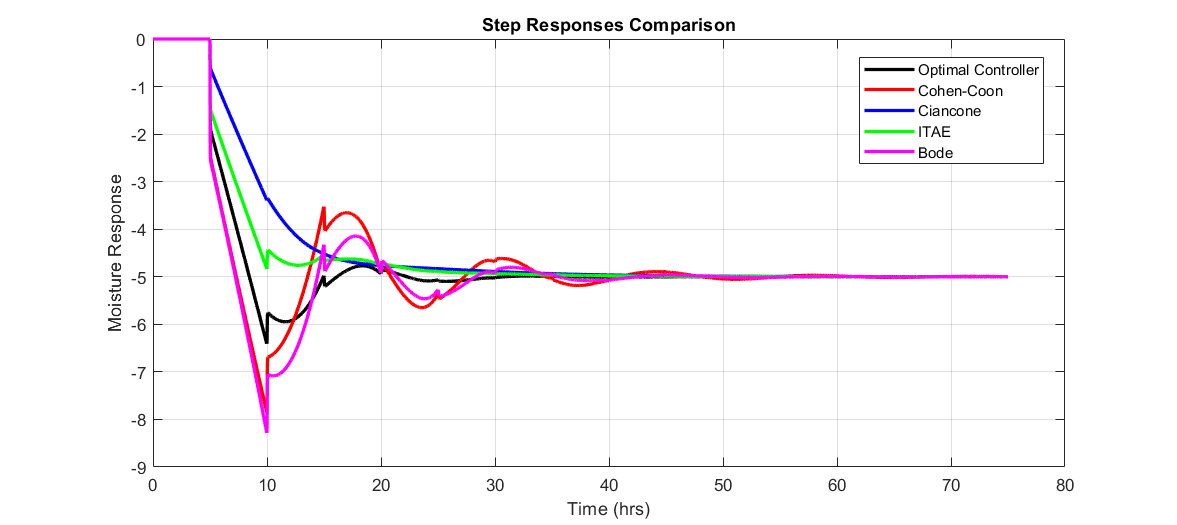
\includegraphics[width=0.7\textwidth]{Figures/figure2-4b.png}
      \caption{Contour Plot of ISE Values for Range of \( K_c \) and \( \tau_I \)}
      \label{fig:figure2_4b}
    \end{figure}

    The results can be summarized as follows:
    \begin{itemize}
        \item \textbf{Cohen-Coon Controller:} The Cohen-Coon controller exhibits a sharp and aggressive response, with a steep initial decrease and a larger negative overshoot. This behavior is likely due to the high values of \( K_p \) and \( K_d \). Additionally, the Cohen-Coon controller takes the longest time to converge, stabilizing after approximately 70 hours.
        \item \textbf{Ciancone Controller:} The Ciancone controller produces an overdamped response, with slower convergence compared to the ITAE and Bode controllers. However, it stabilizes faster than the Cohen-Coon controller, taking approximately 40 hours to converge.
        \item \textbf{ITAE Controller:} The ITAE controller demonstrates smooth and stable performance, with minimal overshoot and faster convergence compared to the Cohen-Coon and Ciancone controllers. It is well-suited for systems requiring rapid settling and stability.
        \item \textbf{Bode Controller:} The Bode controller exhibits a similar shape to the ITAE controller but has slightly more overshoot and oscillations. While it converges quickly, it is less stable than the ITAE controller.
        \item \textbf{Optimal Controller:} The optimal controller, with \( K_c = -1.2 \) and \( \tau_I = 7.5 \), achieves the lowest ISE and provides the smoothest response. It balances speed, stability, and minimal overshoot, making it the best choice among the designs.
    \end{itemize}

    

  \end{enumerate}

\end{enumerate}

\end{document}
